% Introduction

\section{Scope of this study}

A growing number of firms are embracing open innovation as a competitive strategy. Not only does this allow them to access external knowledge resources, it also enables them to profit from internally developed knowledge by making it available to other firms. However, little is known about the role of tacit knowledge in open innovation, which is surprising considering tacit knowledge guides the learning and thought processes that produce novel ideas. This study attempts to fill this gap in knowledge by examining tacit knowledge sharing in three open innovation collaborations. Particular attention is given to how people are motivated to share tacit knowledge and what different patterns of knowledge brokerage reveal about power-relations in each case. \medskip

\section{Background}

\subsection{Defining innovation}

This study defines innovation as \enquote{the development and implementation of new ideas by people who, over time, engage in relationships with others within an institutional and environmental context} \citep{van1986central}. So long an idea is perceived as new to the people involved, it is an innovation even though others may see it as an imitation of something that exists elsewhere \citep{van1986central}. From a business perspective, innovation is about renewal of the business so it can enhance its ability to create value and remain competitive \citep{schumpeter1950capitalism}. Failure to innovate places a firm's ability to survive and prosper at risk \citep{bessant2005managing}. \medskip 

\subsection{Trend towards open innovation}

Firms are finding it harder to compete in the knowledge-based economy. Much of this can be attributed to the ever-increasing technical complexity of products, processes, and services that demand levels of knowledge beyond what most firms possess or can develop in a market-relevant time-frame. Many firms are turning towards open innovation to counter this \citep{enkel2009open,bessant2013innovation,stanko2017under}. Open innovation is formally defined as a distributed innovation process based on carefully managed knowledge flows across firm boundaries using mechanisms as per the firm's business model\footnote{The term \enquote{business model} is defined as \enquote{the chosen system of inputs, business activities, outputs and outcomes that aims to create value over the short, medium, and long term} \citep{gould2013business}}. The business model helps a firm determine which inflows of knowledge can fuel innovation, and which knowledge should be released to other organisations \citep{chesbrough2017future}. \medskip 

According to the resource-based view of the firm, competitive advantage stems from the application of tangible and intangible resources available to the firm \citep{wernerfelt1984resource,peteraf1993cornerstones}. Sustained competitive advantage can be achieved if these resources are valuable, rare, inimitable, and non-substitutable \citep{barney1991firm}. A derivative of the resource-based view is the knowledge-based view of the firm, which considers knowledge to be the most important resource of a firm \citep{grant1996toward}. The knowledge-based view emphasises the importance of having effective processes for transferring knowledge across organisational boundaries \citep{kogut1992knowledge,grant1996toward}. This requires a relational view that focuses on the social structures, routines, and processes for knowledge exchange \citep{dyer1998relational,nahapiet1998social}. Open innovation substantiates the relational view of competitive advantage. The business model that underpins open innovation explains how relational rents can be generated from knowledge sharing activities \citep{durst2013success}. \medskip

Key benefits of open innovation include early access to new technology, sharing of risk, reduced costs of development, better customer acceptance of products or services, and enhanced ability to continuously innovate \citep{ye2013exploring}. Because distributed innovation processes are hard to observe and imitate, open innovation is a useful strategy for sustaining competitive advantage \citep{barney1991firm,lichtenthaler2011open}. \medskip

\subsection{Open innovation processes}

Open innovation can be described in terms of inbound, outbound and coupled innovation processes \citep{chesbrough2006beyond,enkel2009open,gassmann2010future}. Figure \ref{fig:oi_process} illustrates how these processes may work in practice. \enquote{Inbound open innovation} enriches a firm’s knowledge base through integrating suppliers, customers and other external actors \citep{xu2013inbound} whereas \enquote{outbound open innovation} refers to the commercial exploitation of knowledge that has been developed in-house \citep{de2016knowledge}. \enquote{Coupled open innovation} focuses on strategic partnerships that encompass both inbound and outbound innovation processes \citep{spithoven2013open}. \medskip

\begin{figure}
	\centering
	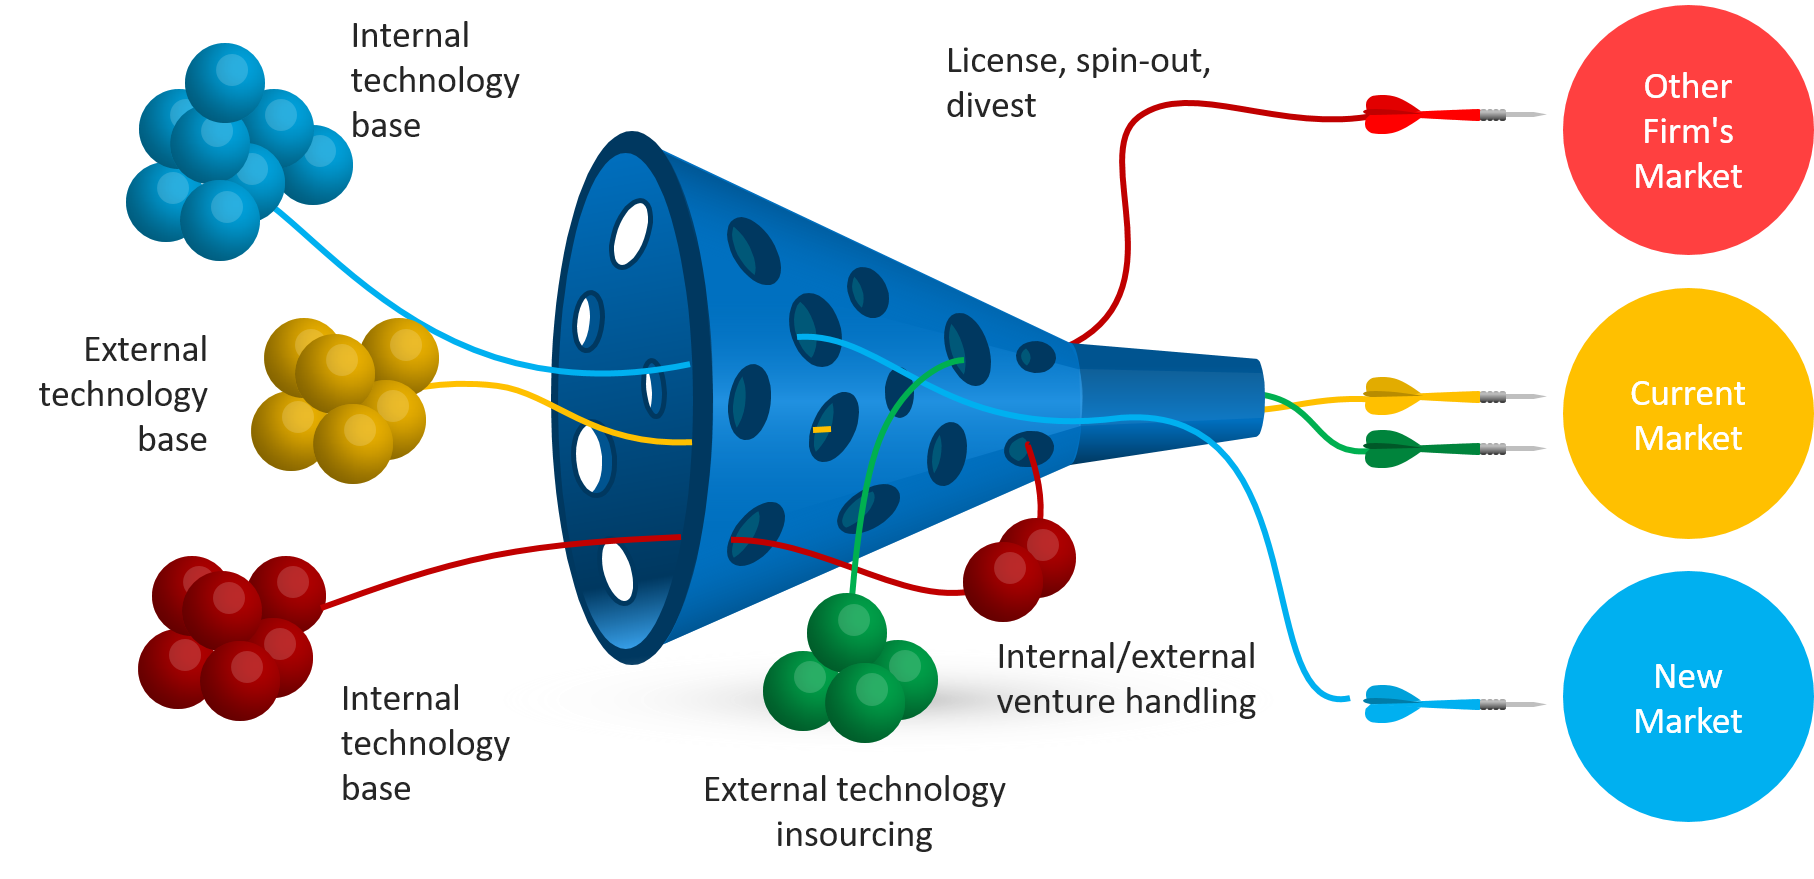
\includegraphics[width=0.9\linewidth]{oi_process_2}
	\caption{Open innovation processes \citep{chesbrough2004open}. Image from SlideModel\texttrademark.}.
	\label{fig:oi_process}
\end{figure}

\subsection{Challenges of open innovation}

Despite its many potential benefits, open innovation presents considerable management challenges \citep{hossain2013open,vanhaverbeke2014surfing}. Transforming the existing business model to support open innovation, changing internal approaches to research and development, building a more open culture, finding suitable organisations to partner with, and managing intellectual property are some of the more pressing challenges \citep{dahlander2010open,sieg2010managerial,lichtenthaler2011your,durst2013success,roper2013externalities,aloini2016structured}. Overcoming relative differences in absorptive capacity between open innovation partners is particularly challenging \citep{vanhaverbeke2007connecting,lakemond2016match}. Tacit knowledge can play a key role in overcoming relative differences in absorptive capacity. However, mobilising tacit knowledge is a challenge in itself \citep{gassmann2004towards,bahemia2010contingent,bogers2011open}. More on the challenges of overcoming absorptive capacity and mobilising tacit knowledge below. \medskip

\subsubsection{Relative differences in absorptive capacity}

Firms need absorptive capacity to bridge cognitive gaps and allow them to capture value from open innovation \citep{vanhaverbeke2007connecting}. Absorptive capacity is defined as the \enquote{ability of a firm to recognise the value of new, external information, assimilate it, and apply it to commercial ends} \citep{cohen1990absorptive}. Relative differences in absorptive capacity between partner firms can impede the flow of knowledge across firm boundaries, contribute to power imbalances, undermine alliance performance, all of which can result in less favourable open innovation outcomes \citep{szulanski1996exploring,lane1998relative,nooteboom2000learning,vanhaverbeke2007connecting,easterby2008absorptive,phelps2012knowledge} \medskip.
 
Though a vast body of research has examined various aspects of absorptive capacity, the concept remains elusive for both researchers and practitioners \citep{duchek2013capturing,omidvar2013revisiting}. Early conceptualisations of absorptive capacity emphasised the importance of prior related knowledge to facilitate associative learning \citep{cohen1990absorptive}. These early conceptualisations paid little attention to the processes that build absorptive capacity \citep{zahra2002absorptive}. More recent conceptualisations treat absorptive capacity as a dynamic capability\footnote{Ordinary capabilities can be thought of as \enquote{do things right} in the core business functions of operations, administration and governance. Dynamic capabilities are about sensing new opportunities, mobilising resources to tackle opportunities, and transforming things \citep{teece2014foundations}} that integrates processes for acquiring, assimilating, transforming, exploiting new knowledge \citep{zahra2002absorptive,todorova2007absorptive,volberda2010perspective,lewin2011microfoundations,marabelli2014knowing}. Absorptive capacity may be treated as a form of organisational learning concerned with new external knowledge, one that involves processes and routines to share, communicate, and transfer individual learning to the group and organisational levels \citep{sun2010examination}. \medskip

Building absorptive capacity is challenging because it cuts across multiple levels and is contingent not only on prior related knowledge and social mechanisms for integrating diverse knowledge, but also on the strength or weakness of appropriability regimes \footnote{Appropriability refers to a firm's ability to prevent knowledge and innovations from being appropriated by other firms. This depends on the features of the core knowledge in innovation (tacit vs. codified) and the efficacy of legal protection for intellectual assets.   \citep{teece1998capturing}Appropriability regime has been defined as the scope in which knowledge and innovations can be protected from imitators .} and nature of power-relations \citep{todorova2007absorptive,easterby2008absorptive,duchek2013capturing}. \medskip 

\subsubsection{Mobilising tacit knowledge}

Past studies of absorptive capacity have emphasised the importance of prior knowledge possessed by individuals and groups. Much prior knowledge is tacit, held either in people's minds or in the form of unwritten rules or practices that guide the collective action of groups \citep{mowery1996strategic,leonard1998role,horvath2000working,burt2007secondhand,nonaka2009perspective,goksel2016can,lichtenthaler2016absorptive}. Tacit knowledge tends to reflect more closely the reality of how work actually gets done \citep{horvath2000working}. \medskip

Knowledge exists on a spectrum where at one extreme, it is almost completely tacit, that is knowledge held in peoples' minds and bodies. At the other extreme, knowledge is almost completely explicit, existing in codified or structured form and accessible to other people \citep{polanyi1966tacit,inkpen1998knowledge,leonard1998role,cavusgil2003tacit}.  \medskip

Tacit knowledge is associated with terms such as \enquote{intuition}, \enquote{skill}, \enquote{know-how}, and \enquote{expertise} used to describe knowledge that refers to an ability to perform work \citep{mcadam2007exploring}. Tacit knowledge is considered critical for innovation as it guides the thought processes that produce novel ideas \citep{leonard1998role,amar2008descriptive}. The most common application of tacit knowledge is problem-solving. People with expertise borne from experience not only are able to recognise the situation in which they find themselves in, but also know which actions might be appropriate for dealing with it \citep{simon1971human,leonard1998role}. Tacit knowledge is also used to reformulate problems or anticipate outcomes in intuitive ways \citep{leonard1998role}. \medskip

Many firms do not appreciate the diversity of their knowledge resources and thus fail to see the potential value and uses of tacit knowledge \citep{nonaka1994dynamic,horvath2000working}. Mobilising tacit knowledge in open innovation requires all parties to fully appreciate tacit knowledge held in people's minds or group practice. This is easier said than done as people are either unaware of the tacit dimension of their knowledge or unable to express what they know, or they are reluctant to give up any advantages their tacit knowledge or know-how affords them \citep{polanyi1966tacit,leonard1998role,eraut2000non}. \medskip

The tacit knowledge that guides the collective action of groups is prone to being discounted or misunderstood by others \citep{burt2007secondhand}. This emphasises the need for people in boundary spanning roles to aid the transfer of diverse and often complex knowledge between groups \citep{tushman1981boundary,allen1984managing,szulanski2003sticky,seidler2008use,meyer2010rise,chesbrough2012open}. Another way to facilitate the transfer of tacit knowledge is through communities of practice \citep{lave1991situated,brown2001knowledge,smith2001role,cox2005communities,easterby2008inter}. These function as a social instrument to create, share and steward knowledge, and they are a pragmatic basis of an organisation’s absorptive capacity and significant sites of innovation \citep{brown1991organizational}. \medskip

\subsubsection{Brokering productive relationships}

Boundary spanners play a key role in open innovation as they broker new relations between otherwise disconnected actors in different organisational networks and facilitate the translation, integration and combination of unfamiliar and distant knowledge \citep{granovetter1973strength,tushman1981boundary,allen1984managing,szulanski2003sticky,burt2004structural,burt2007secondhand,seidler2008use,meyer2010rise,chesbrough2012open}. \medskip

Management efforts to create or widen existing inter-organisational networks may be frustrated by people reluctant to form new ties, facilitate third-party ties, or otherwise change their existing networks \citep{davis2010agency}. Not-invented-here and not-shared-here (also referred to as not-sold-here) syndromes can also stymie knowledge exchange \citep{lichtenthaler2006attitudes,lichtenthaler2011your,de2014neither,podmetina2015skills,chesbrough2017future}. Not-invented-here syndrome refers to resistance within a firm against externally developed knowledge \citep{katz1982investigating,hussinger2011search,antons2015opening}. Not-shared-here syndrome is a negative attitude towards external exploitation of internally developed knowledge \citep{chesbrough2003open,lichtenthaler2006attitudes,de2014neither}. \medskip

Figuring out ways to overcome negative attitudes towards knowledge sharing is essential to allow the formation of new productive relationships that enable knowledge to be recombined in unique and valuable ways \citep{uzzi1997social,nahapiet1998social,obstfeld2005social,lane2006reification,davis2010agency,meyer2010rise}.\medskip

\section{Research opportunity}

The extent to which tacit knowledge helps bridge cognitive gaps is poorly understood. Research into brokerage of tacit knowledge is also lacking. This is hardly surprising, given tacit knowledge is difficult to characterise let alone measure \citep{zander1995knowledge,cavusgil2003tacit}. There is little doubt that tacit knowledge has a significant influence on a firm's absorptive and innovative capacity, and warrants much more attention than it has received so far. \medskip

\subsection{Exploring motivational factors}

Managing the flow of tacit knowledge across organisational boundaries is confounded by the fact that tacit knowledge sharing cannot be mandated but happens through volition or free will \citep{polanyi1966tacit}. Moreover, tacit knowledge can only be shared through direct observation, either via face-to-face social interaction or by video demonstrations \citep{haldin2000difficulties,koskinen2003tacit}. Tacit knowledge is not something that is transferred. Rather, tacit knowledge is interpreted within a specific context. Face-to-face social interaction is considered the richest medium because it allows immediate feedback to check understanding and correct interpretations \citep{koskinen2003tacit}. \medskip

Since tacit knowledge requires significant effort to communicate, people need to be sufficiently motivated to seek out or share tacit knowledge \citep{leonard1998role}. Past studies show a significant and positive relation between an individual's level of intrinsic motivation and the amount of tacit knowledge they share \citep[e.g.][]{osterloh2000motivation,kaser2001knowledge,smith2001role}. While these studies highlight the importance of individual motivation, the social processes underpinning tacit knowledge sharing and how this impacts open innovation are not well understood. This indicates a need to investigate how individual motivation shapes knowledge sharing relations. \medskip

\subsubsection{Unpacking power-relations}

It is often stated that \enquote{knowledge is power} yet little attention has been given to power and power-relations in the knowledge management literature \citep{heizmann2015power}. The current power literature is dominated by two contrasting views of power, namely \enquote{power as domination}, also referred to as \enquote{power-over}, and \enquote{power as empowerment}, often characterised as \enquote{power-to} \citep{haugaard2012rethinking}. Sharing tacit knowledge is essentially all about empowering others so they can perform work more independently and confidently. \medskip

The network perspective treats power as inherently relational \citep{ibarra1993network}. How an actor is embedded in a social network either imposes constraints on the actor or presents the actor with opportunities \citep{burt1992structural,simpson2011network}. Actors with fewer constraints and more opportunities occupy favourable structural positions. Being in a favoured position means that an actor may extract better bargains in exchanges, have greater influence, and be a focus for deference and attention from those in less favoured positions \citep{burt1992structural,hanneman2005introduction,simpson2011network}. \medskip

Actors in a knowledge network serve both as keepers of knowledge and as agents that seek out, communicate, and create knowledge \citep{phelps2012knowledge}. One can assess how actors exercise power by examining patterns of brokerage in knowledge sharing networks. Brokerage may be defined as the \enquote{behaviour by which an actor influences, manages, or facilitates interactions between other actors} \citep{obstfeld2014brokerage}. This definition allows brokerage to be seen in terms of \enquote{power-over} and \enquote{power-to}. \citet{obstfeld2014brokerage} describe three strategic orientations to brokerage: \emph{conduit brokerage} is about a third-party who transfers information, knowledge, or other resources between two disconnected parties. The broker mediates rather than moderates the relationship between two others and may help them synthesise new knowledge. With \emph{tertius gaudens brokerage}, the broker aims to exploit differences between two parties by either keeping them apart or playing one against another. In contrast, \emph{tertius iungens brokerage} is about a third-party who introduces two otherwise disconnected parties to each other and encourages them to collaborate (Figure \ref{brokerage}). \medskip 

\begin{table}[]
\small
\centering
\caption{Three forms of brokerage process. Reproduced from \citet{obstfeld2014brokerage}.}
\label{brokerage}
\begin{tabularx}{\textwidth}{p{3.5cm}p{3.5cm}p{3.5cm}p{3.5cm}}
	\toprule
	& \multicolumn{1}{c}{Conduit} & \multicolumn{1}{c}{Tertius Gaudens} & \multicolumn{1}{c}{Tertius Iungens} \\ \midrule
	& \begin{minipage}{.2\textwidth} \centering 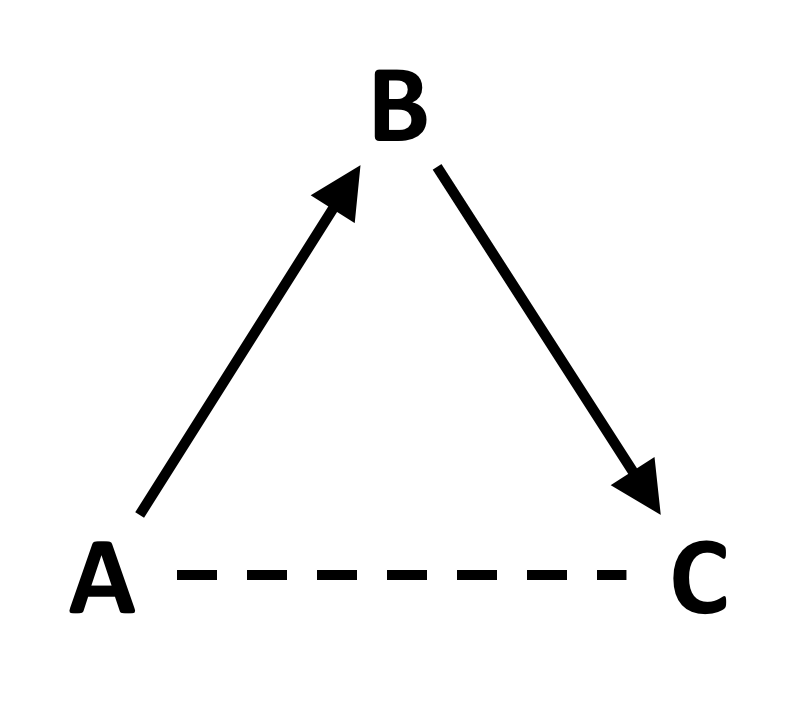
\includegraphics[width=0.7\linewidth]{Images/CDT_brokerage} \end{minipage}  & \begin{minipage}{.2\textwidth} \centering 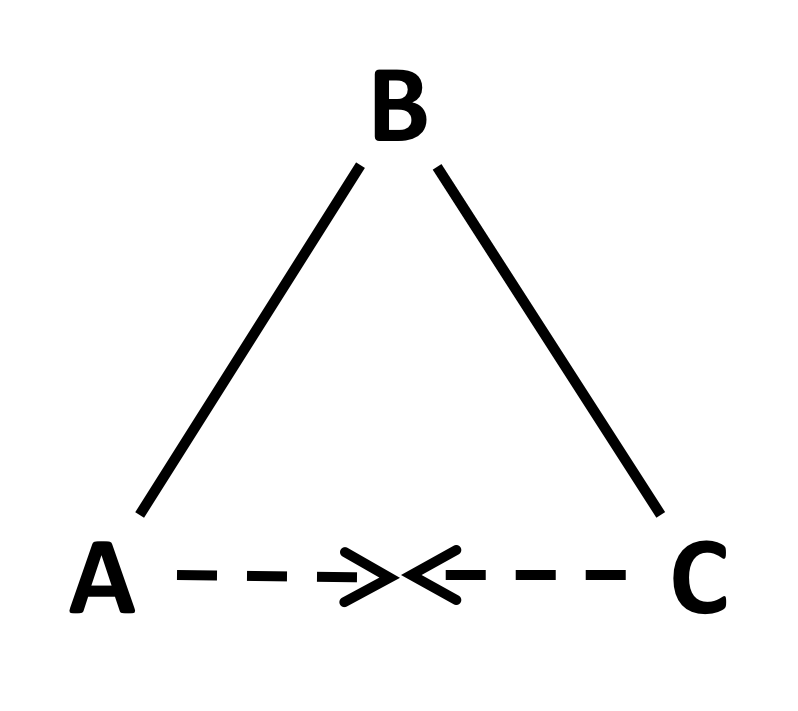
\includegraphics[width=0.7\linewidth]{Images/TG_brokerage_1} \end{minipage}  & \begin{minipage}{.2\textwidth} \centering 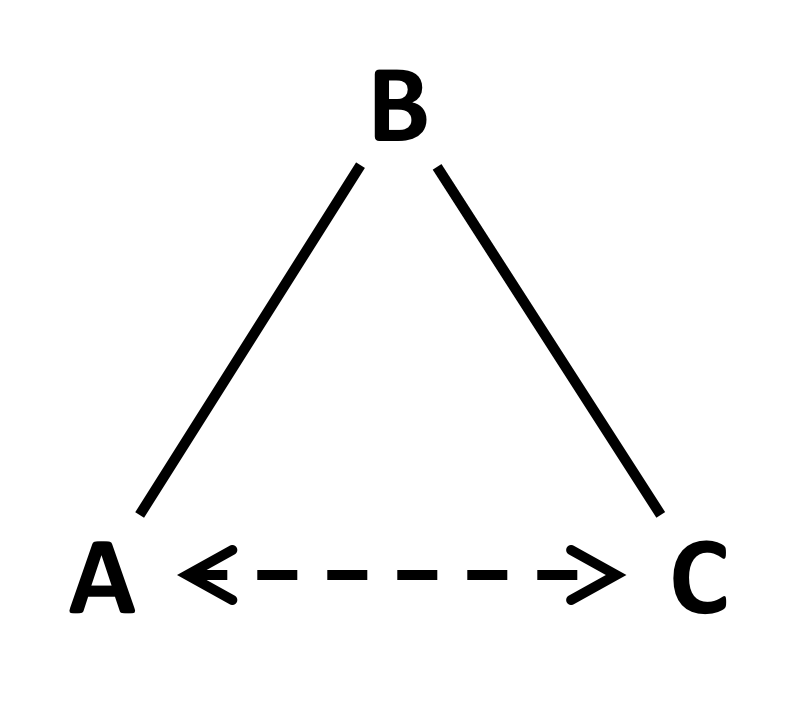
\includegraphics[width=0.7\linewidth]{Images/TI_brokerage} \end{minipage}   \\
	&  & \begin{minipage}{.2\textwidth} \centering 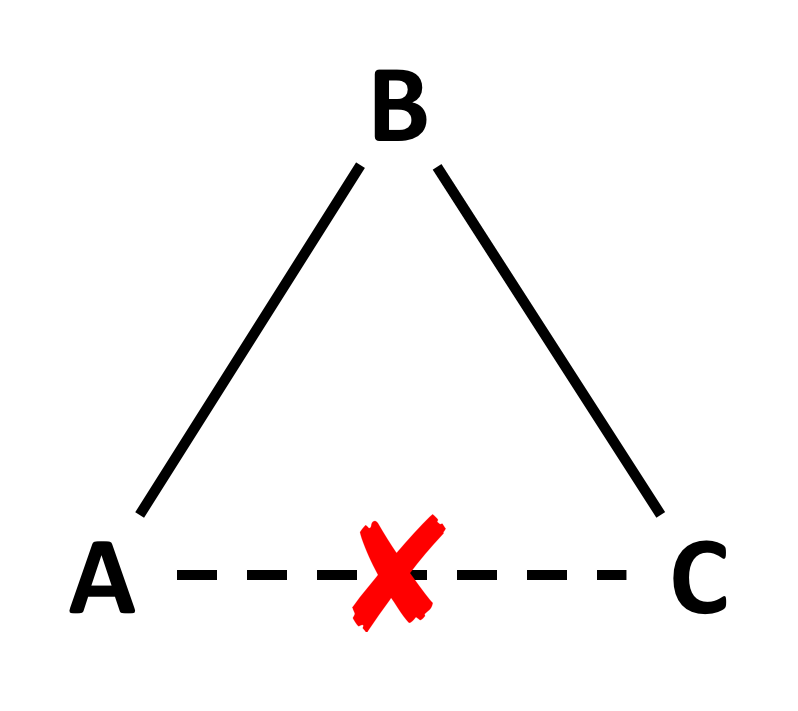
\includegraphics[width=0.7\linewidth]{Images/TG_brokerage_2} \end{minipage}  &  \\ \midrule
	Open network\\(absence of A-C tie) & B transfers information, knowledge, or other resources between A and C where A and C have no prospect of meeting & B plays A and C against one another or keeps A and C apart & B introduces A and C where A and C have no prior tie \\ \midrule
	Closed Network\\(presence of A-C tie) & B facilitates transfer between A and C and may help synthesise new knowledge & B cultivates conflict,,competition, or separation between A and C (divide et impera) & B coordinates new collaborative action between A and C \\ \bottomrule
\end{tabularx}
\end{table}

From an open innovation perspective, \emph{tertius iungens brokerage} is quite important, especially in the early stages of collaboration, when many actors do not know fellow collaborators in partner organisations. Not only that, knowledge held by third parties is also likely to be unfamiliar. Once ties have been established through \emph{tertius iungens brokerage}, \emph{conduit brokerage} is needed to help synthesise and transform knowledge into novel ideas \citep{fleming2007collaborative,lingo2010nexus,quintane2016brokers}. \citet{gould1989structures} describe \emph{conduit brokerage} in terms of \emph{coordination}, \emph{liaison}, \emph{itinerant}, \emph{representative}, and \emph{gatekeeper} roles (Figure \ref{gf_params}). Each role expresses a different power dynamic and one should be able to use the relative proportion of each role to characterise power-relations in open innovation collaborations. \medskip

\begin{table}[]
	\small
	\centering
	\caption{Gould-Fernandez brokerage roles}
	\label{gf_params}
	\begin{tabularx}{\textwidth}{@{}lcl@{}}
		\toprule
		\multicolumn{1}{c}{Role} & \multicolumn{1}{c}{Graphic} & \multicolumn{1}{c}{Explanation} \\ \midrule
		Liaison (b\textsubscript{O})			&  \begin{minipage}{.2\textwidth} \centering 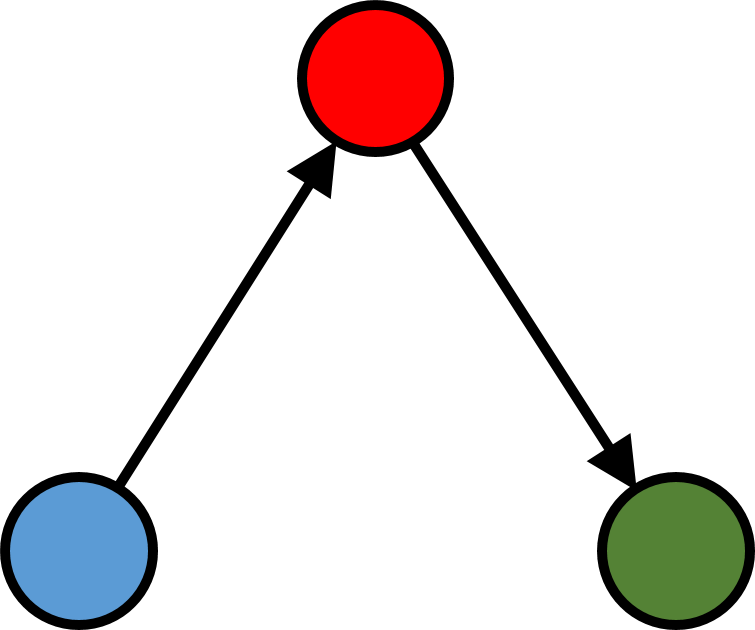
\includegraphics[width=0.4\linewidth]{Images/b_O} \end{minipage}	& \begin{tabular}[c]{l}Broker mediates contact between two\\ individuals from different groups,\\ neither of which is the group to\\ which he or she belongs.\end{tabular}\\ [10ex]
		Representative  (b\textsubscript{IO})	& \begin{minipage}{.2\textwidth} \centering 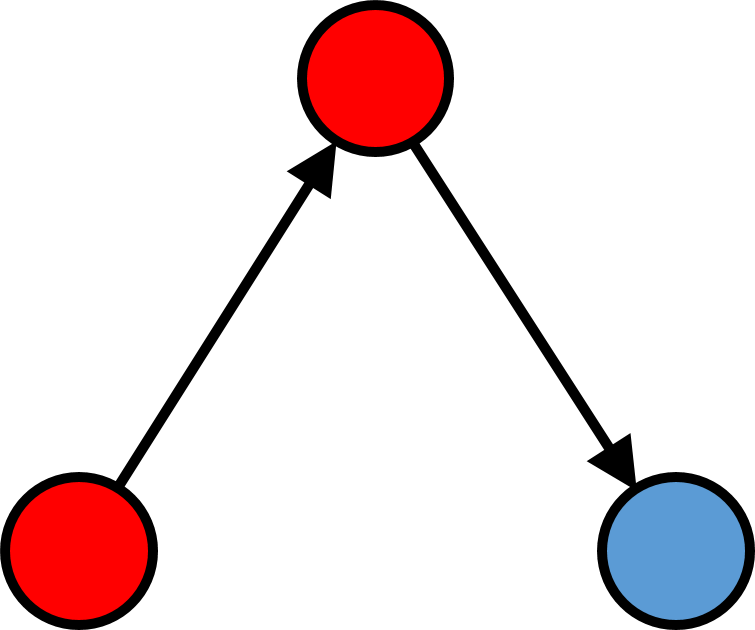
\includegraphics[width=0.4\linewidth]{Images/b_IO} \end{minipage}   & \begin{tabular}[c]{l}Broker mediates an outgoing contact\\ from an in-group member to an\\ out-group member.\end{tabular}\\ [10ex]
		Gatekeeper (b\textsubscript{OI})		& \begin{minipage}{.2\textwidth} \centering 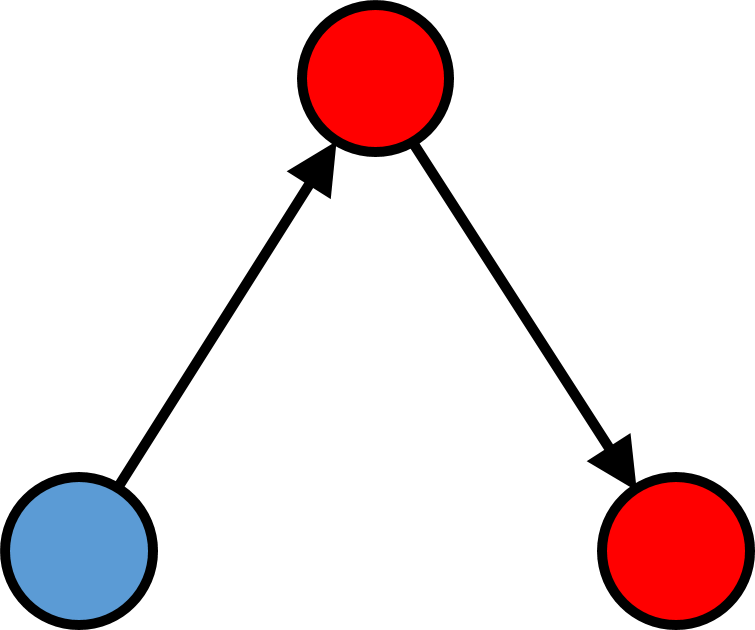
\includegraphics[width=0.4\linewidth]{Images/b_OI} \end{minipage}   & \begin{tabular}[c]{l}Broker mediates an incoming contact\\ from an out-group member to an\\ in-group member. \end{tabular}\\ [10ex]
		Itinerant broker (w\textsubscript{O})	&  \begin{minipage}{.2\textwidth} \centering 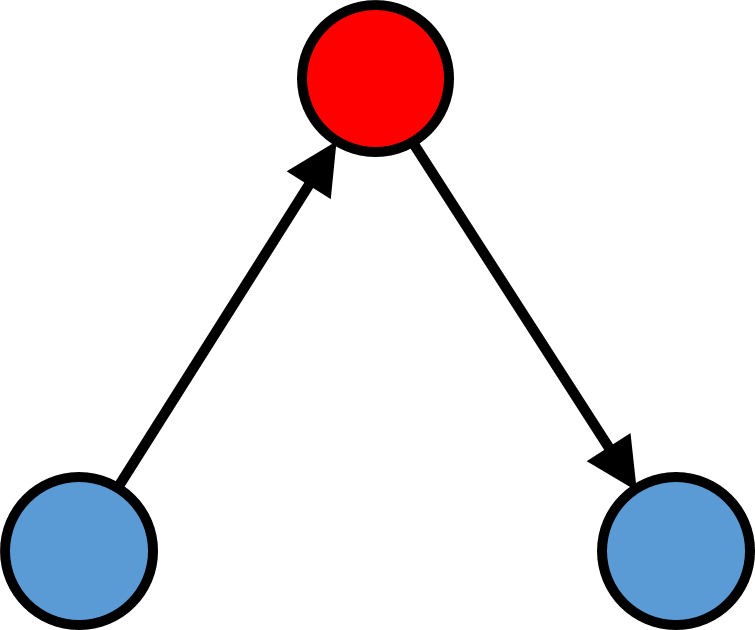
\includegraphics[width=0.4\linewidth]{Images/w_O} \end{minipage}   & \begin{tabular}[c]{l}Broker mediates contact between two\\ individuals from a single group to\\ which he or she does not belong. \end{tabular}\\ [10ex]
		Coordination (w\textsubscript{I})		& \begin{minipage}{.2\textwidth} \centering 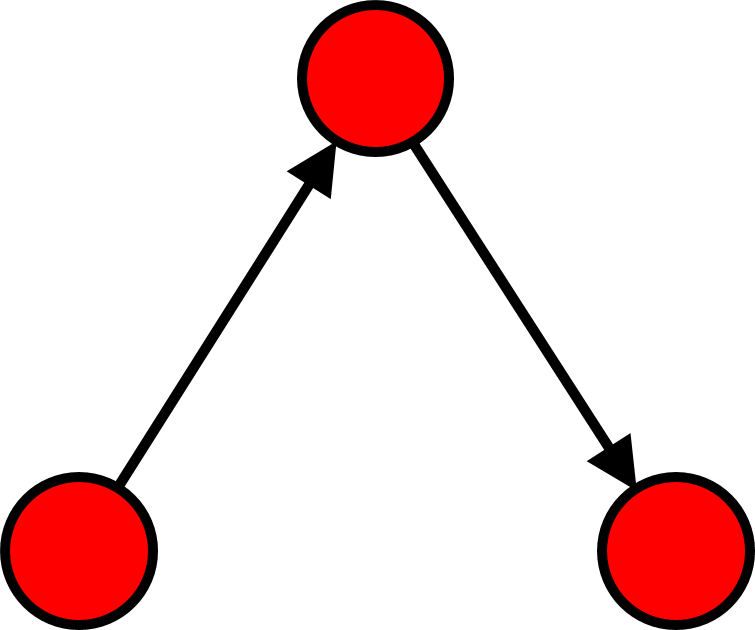
\includegraphics[width=0.4\linewidth]{Images/w_I} \end{minipage}    & \begin{tabular}[c]{l}Broker mediates contact between two\\ individuals from his or her own\\ group. \end{tabular}\\ 
		\bottomrule
	\end{tabularx}
\end{table}
 
\section{Study objectives}

This study employs mixed methods social network analysis assess tacit knowledge sharing in three open innovation partnerships. Particular attention is given to how people are motivated to share tacit knowledge and what different patterns of knowledge brokerage reveal about power-relations in each case. The overarching research question tackled in this study is \enquote{how do psychological and social factors shape tacit knowledge sharing in open innovation?}. This question is answered by addressing four specific sub-questions: \medskip

\begin{enumerate}
	\item How important is tacit knowledge sharing for idea generation in open innovation partnerships?
	\item To what extent does the level and type of personal motivation predict tacit knowledge sharing in open innovation partnerships?
	\item What does the configuration of tacit knowledge networks reveal about power-relations in open innovation partnerships?
	\item How does organisational culture contribute to tacit knowledge sharing in open innovation partnerships?
\end{enumerate}

The mixed methods social network analysis uses statistical modelling to (a) assess how individual attributes, such as level and type of personal motivation, educational background, and work experience drive the emergence of tacit knowledge sharing relations, and (b) examine what patterns of brokerage reveal about power-relations in tacit knowledge networks. This modelling is complemented by semi-structured interviews that capture the industrial, organisational, and cultural contexts governing the emergence of collaborative social structures. \medskip  

\section{Research contribution}

This study advances knowledge in two ways. Firstly, the study provides fresh insight into how tacit knowledge sharing facilitates learning and idea generation in open innovation partnerships. Secondly, it breaks new ground by examining how knowledge brokerage varies according to the amount of tacit knowledge being exchanged and what this means in terms of power-relations. Both contributions should contribute to more effective management of knowledge flows in open innovation. \medskip


\section{Document structure}

This document is organised into ten chapters:

\begin{itemize}
	\item[Chapter Two] reviews key psychological and social theories that can be used to assess knowledge sharing behaviour. These include the \emph{Theory of Planned Behaviour}, \emph{Self-Determination Theory}, \emph{Structural Hole Theory}, and recent contributions to \emph{Brokerage Theory}.
	\item[Chapter Three] characterises salient features of social networks and introduces exponential random graph models, an advanced social network analysis technique used in this study.
	\item[Chapter Four] explains the convergent parallel mixed method research design used in this study. 
	\item[Chapter Five] highlights the unique characteristics of each open innovation partnership.
	\item[Chapter Six] reports on how the type and level of individual motivation shapes tacit knowledge sharing relations in each partnership.
	\item[Chapter Seven] describes the different patterns of knowledge brokerage encountered in each partnership and what these reveal about power-relations.
	\item[Chapter Eight] discusses the implications for managing tacit knowledge flows in open innovation.
	\item[Chapter Nine] summarises the key findings of this study and reflects on some key lessons learned as this study unfolded.        
\end{itemize}
